\documentclass{article}
\usepackage[utf8]{inputenc}
\usepackage[dvipdfmx]{hyperref}
\usepackage{fancyhdr}
\usepackage{caption, floatrow}

\usepackage[dvipdfmx]{graphicx}

\usepackage{mathtools}
\renewcommand{\theequation}{eq. \arabic{equation}}


\usepackage[
  style=numeric,
  citestyle=numeric,
  url=true,
  doi=false,
  isbn=false
  ]{biblatex}
\addbibresource{main.bib}


\DeclareNewFloatType{graph}{placement=H, name=Graph}
\floatsetup[graph]{capposition=bottom}


% contents below
% ------------------------------------------------------------------------------

\pagestyle{fancy}
\fancyhf{}
\rhead{Rikuo Hasegawa}
\chead{UPCSE PHYSICS Short Lab Report}
\lhead{\today}
\rfoot{p. \thepage}

\title{Refractive Index}
\author{ Rikuo Hasegawa
  \\ Tutorial Group: C
  \\ Lab Group: C2 }

\begin{document}

\maketitle
\thispagestyle{fancy}
\vspace*{\fill}
\parbox{\linewidth}{\centering%
Date of Experiment: February 20th, 2019
}
\newpage


\section{Introduction}
\paragraph{}
In this experiment our goal was to measure the refractive index of a glass prism by measuring the minimum angle of deviation when shining a beam of light through the prism and the angle of the prism.

\section{Theory}
\paragraph{}
When shining a light through a prism, the angle of deviation ($D$) is the angular difference between the path which would be taken by the beam of light had the prism not been there, with the actual path the beam takes when it goes through the prism.

There is one minimum angle of deviation for a given prism for a given wavelength of light. If the wavelength and prism shape are fixed, this is dependent on the angle of incidence of the beam to the prism.

In order to find the angle $A$ of the prism, we shine a beam onto a vertex of the triangle on the prism as in Figure \ref{fig:prism}

\begin{figure}
  \includegraphics{./img/2A.pdf}
  \caption{Figure showing rays of light reflecting off prism.}
  \label{fig:prism}
\end{figure}

This is not very intuitive, so a detailed explanation is indicated in Figure \ref{fig:proof}. Assuming there is an angle of incidence going through the vertical line from the vertex to the base of the triangle, $\theta$, we can see that each side of the prism adds or subtracts $\frac{A}{2}$ to this angle. When the beam hits the prism, it reflects at an angle $\frac{A}{2} \pm \theta$ which combines with the angle $A$ of the prism and cancels out the $\theta$s to become $2A$.

\begin{figure}[h]
  \includegraphics[width=100mm]{./img/proof.pdf}
  \caption{Rays of light equal $2A$ regardless of small asymmetries in prism orientation.}
  \label{fig:proof}
\end{figure}

From Figure \ref{fig:prism}, we can see that the beams reflected off the prism will have an angle of $2A$ between them.

If an equilateral triangular prism has an angle $A$, the index of refraction $\mu$ can be given by \eqref{eq:mu} \autocite{UPCSE2018}

\begin{equation}\label{eq:mu}
  \mu = \cfrac{
    \sin{\cfrac{A+D}{2}}
  }{
    \sin{\cfrac{A}{2}}
  }
\end{equation}

\section{Experimental Equipment and Method}
\subsection{Apparatus}

Our apparatus is shown in Figure \ref{fig:apparatus}.

It consists of the following main components:
\begin{itemize}
  \item Sodium Lamp
  \item Collimator to filter the lamp into a beam
  \item Glass prism on turntable
  \item Telescope on a radial vernier scale
\end{itemize}

\begin{figure}[h]
  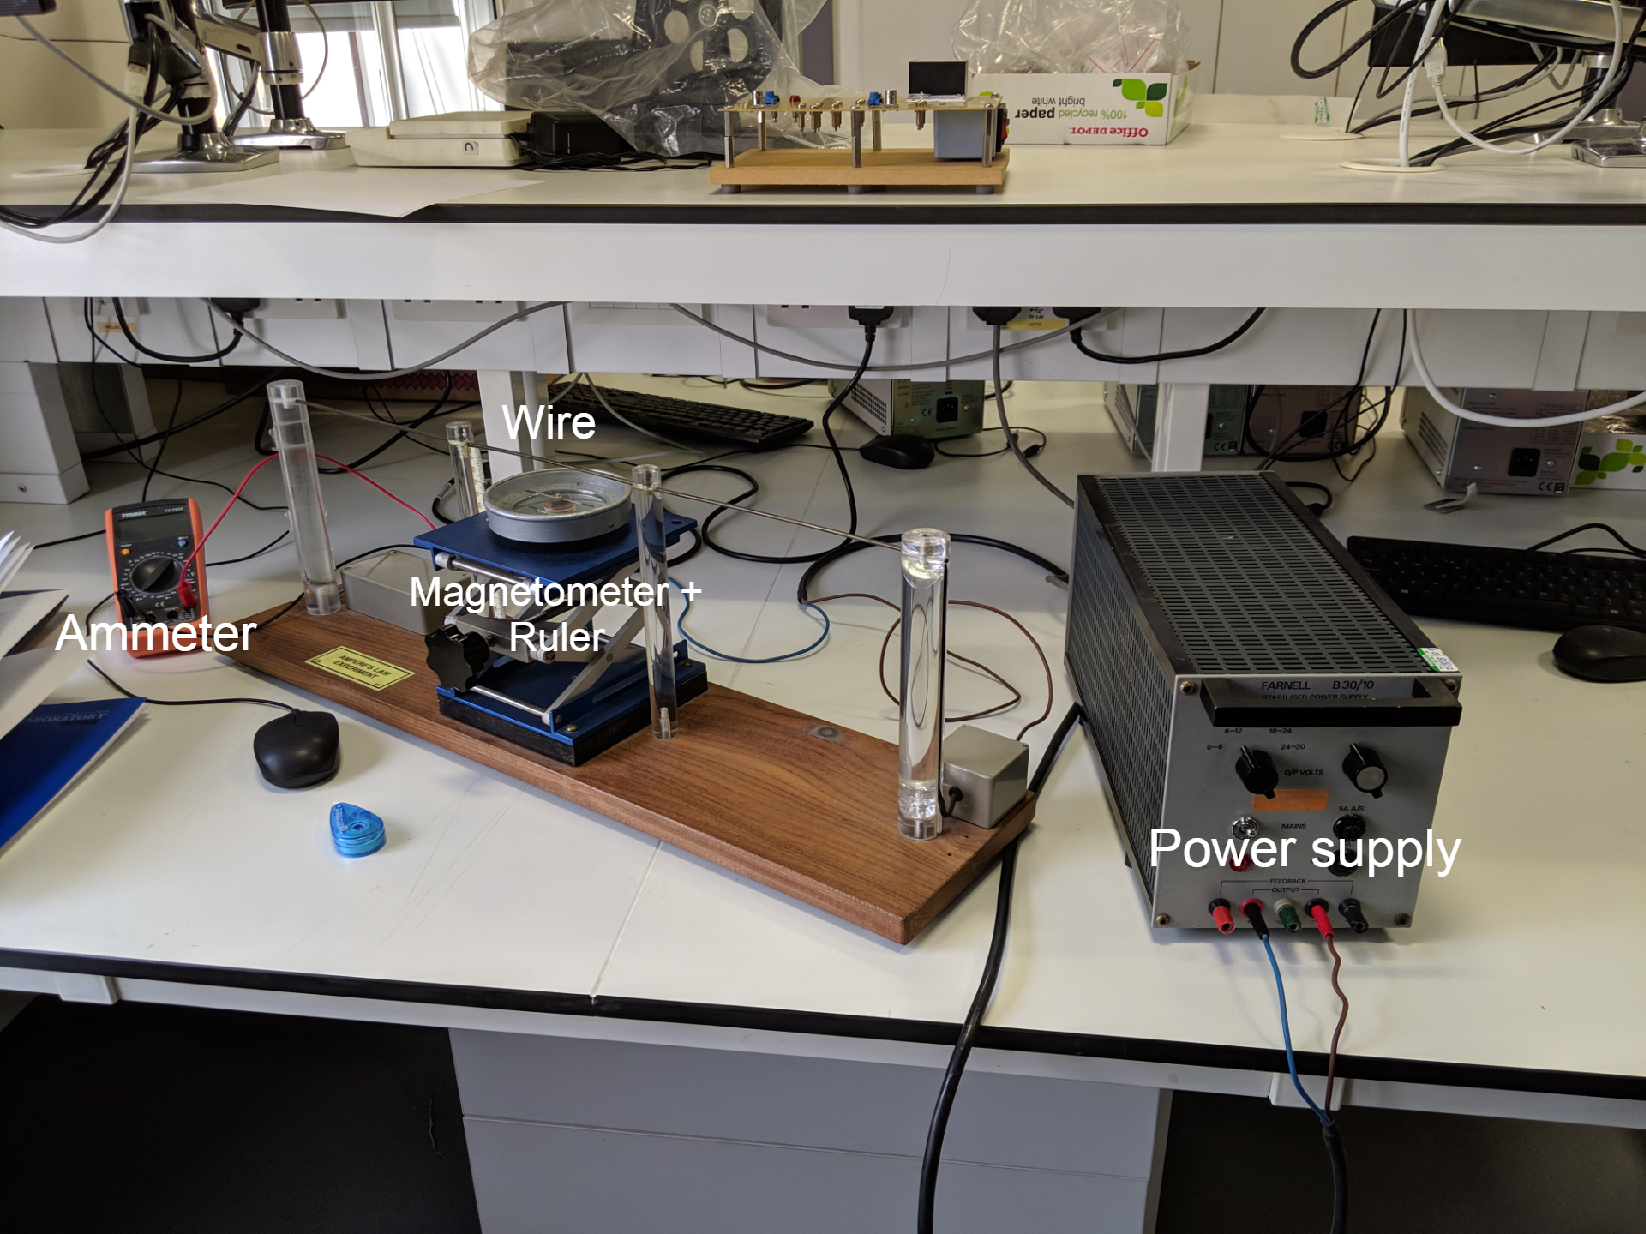
\includegraphics{./img/apparatus.pdf}
  \caption{Apparatus}
  \label{fig:apparatus}
\end{figure}

The uncertainty on the vernier scale is 0.5 minutes, or $1/120$ degrees.

\subsection{Protocol}
The protocol is described below:

\begin{itemize}
  \item Turn on the sodium lamp and calibrate the telescope and collimator so the image is clear and the beam is as thin as possible.
  \item Find the angle where the beam would be if there was no prism by finding the beam when it is not going through the prism and centering it on the crosswires of the telescope.
  \item Place the prism so it intersects with the beam. Find the refracted beam with the telescope.
  \item Adjust both the telescope and angle of the prism until you find the minimum angle of deviation from the straight line position.
  \item Measure.
\end{itemize}

The protocol for finding the angle $A$ of the prism is similar to the one above, but we place the prism such that the beam hits a vertex of the prism, and we measure the angular difference between the two reflected beams.

\section{Results}

Our results for the measurement of $D$ and $A$ are shown in Table \ref{tb:D} and Table \ref{tb:A} respectively.

\begin{table}
  \includegraphics[width=\textwidth]{./img/D.pdf}
  \caption{Measurements of angle of deviation $D$}
  \label{tb:D}
\end{table}

\begin{table}
  \includegraphics[width=\textwidth]{./img/A.pdf}
  \caption{Measurements of angle of prism $A$}
  \label{tb:A}
\end{table}

\section{Uncertainty Analysis}

We will look at \eqref{eq:mu} to get our measurement of the refractive index of our prism. Since we do not have any outliers in our data, we will look to finding the uncertainty by examining the range of values which $\mu$ can take to estimate our random error.

$$
\mu_{max} = 1.57
$$

$$
\mu_{min} = 1.52
$$

Thus, we will use \eqref{eq:half_range} to find our estimate of the value of $\mu$ with the uncertainty.

\begin{equation}\label{eq:half_range}
  \mu = \frac{1}{2}(\mu_{max} + \mu_{min}) \pm \frac{1}{2}(\mu_{max} - \mu_{min})
\end{equation}

$$ \mu = 1.55 \pm 0.025 $$

\section{Discussion and Conclusion}

We know the true refractive index of glass to be in the range of 1.5 ~ 2.0 \autocite{mohr_2016}. Our results agree with this and we can conclude we may have correctly measured the refractive index of our prism.

If our glass is a material which has a fairly high refractive index for glass, we may have some systematic errors in our experiment but it is unlikely to be the case. If it is the case, some probable causes for this could be from the prism not being completely transparent and uniform. Another possible cause would be that we did not have a clamp to fix our prism in place, so there may have been minute vibrations which caused the prism to move as we took measurements.

\printbibliography
\end{document}
